\newpage
\section{Παλινδρόμησή}
Η παλινδρόμηση είναι μια στατιστική τεχνική η οποία περιγράφει την σχέση που έχουν μία ή
περισσότερες ανεξάρτητες μεταβλητές με μία εξαρτημένη, προσαρμόζοντας μία γραμμή
(παλινδρόμησης) στα δεδομένα. Με αυτή την τεχνική μπορούμε κυρίως να κάνουμε
προβλέψεις για καινούργια δεδομένα ή να συγκρίνουμε διάφορα μοντέλα όπου το καθένα
έχει διαφορετικές μεταβλητές, είτε προς τον αριθμό είτε προς τις μεταβλητές αυτές κάθε
αυτές.

Οι γραμμικές παλινδρομήσεις προσαρμόζουν μία ευθεία γραμμή στα δεδομένα ενώ
οι λογαριθμική/λογιστική (\en{logistic}) και οι μη γραμμικές προσαρμόζουν μία κυρτή γραμμή. Ως
μεταβλητές μπορούν να χρησιμοποιηθούν είτε συνεχή (βάρος, ύψος) είτε διακριτά δεδομένα
(φύλο, ύπαρξη μετάλλαξης ή όχι).

Η παλινδρόμηση έχει ένα ευρύ πεδίο χρίσης, από το πεδίο
των οικονομικών για πρόβλεψη μεταβολών στο χρηματιστήριο και των πωλήσεων, μέχρι και
το πεδίο της υγείας, όπου και θα επικεντρωθούμε σε αυτή την εργασία, για ανάλυση και
πρόβλεψη ασθενειών σε σχέση με κάποια βιολογικά δεδομένα, όπως βιοχημικά, γενετικά,
φυσιολογίας και άλλα. Μερικά είδη παλινδρόμησης είναι:
\begin{itemize}
    \item Απλή γραμμική (συνεχή και διακριτών στοιχείων (\en{t-test/ANOVA}) )
    \item Πολλαπλή παλινδρόμηση
    \item Πολυωνυμική
    \item Λογαριθμική ή λογιστική (\en{Logistic})
    \item Γκαουσιανή
\end{itemize}

\begin{figure}[H]
    \centering
    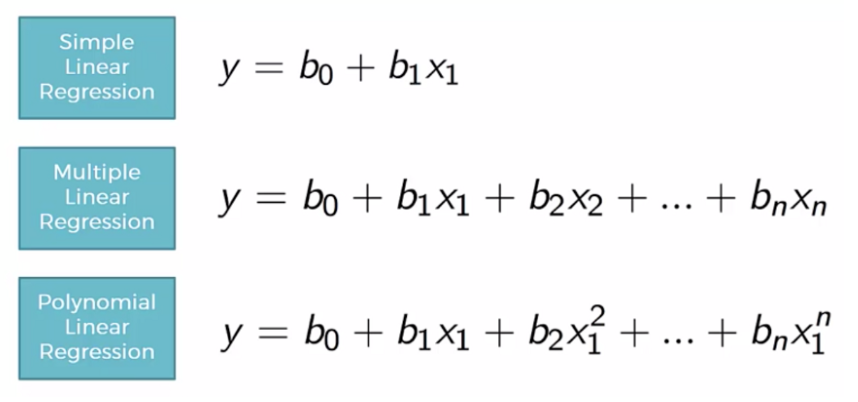
\includegraphics[width=1\textwidth]{images/Regression.png}
    \caption{Είδη παλινδρόμησης}
\end{figure}
\subsection{Γραμμική Παλινδρόμηση}
Η ποιο απλή και ευρέως χρησιμοποιούμενη τεχνική παλινδρόμησης είναι η γραμμική. Όπως
υποδεικνύει το όνομα της η γραμμική παλινδρόμηση συσχετίζει μία ανεξάρτητη με μία
εξαρτημένη μεταβλητή με μία γραμμική σχέση προσαρμόζοντας μία ευθεία γραμμή
παλινδρόμησης πάνω στα δεδομένα. Η ευθεία δίνεται από την σχέση:
$$y=ax+b+c$$
\begin{figure}[H]
    \centering
    \begin{tikzpicture}
        \begin{axis}[xmin = 0, xmax=5, ymin=0, ymax=5, xtick=\empty, ytick=\empty, axis lines=left, scatter/classes={
            b={mark=o,blue}
        }]
            \addplot[scatter, only marks, scatter src=explicit symbolic] coordinates {
                (0.5,2.3) [b]
                (1,3.1) [b]
                (2,3.8) [b]
                (3,5.2) [b]
                (4,5.7) [b]
                (1.5,3.7) [b]
                (2.5,4.6) [b]
                (3.2,5) [b]
            };
            \addplot[red] {x+2};
        \end{axis}
    \end{tikzpicture}
    \caption{Γραμμική παλινδρόμηση}
\end{figure}
όπου:
\begin{description}
    \item[$y$ :] εξαρτημένη μεταβλητή (\textlatin{dependent variabl}e)
    \item[$x$ :] ανεξάρτητη μεταβλητή (\textlatin{Independent / explanatory variable or regressor})
    \item[$a$ :] κλίση της ευθείας (\textlatin{slope})
    \item[$b$ :] σημείο τομής με τον άξονα $y$ ($y$ – \textlatin{intercept})
    \item[$c$ :] σφάλμα παλινδρόμησης (\textlatin{regression residual / error})
\end{description}

Η ευθεία αυτή προσαρμόζεται στα δεδομένα με την χρήση της τεχνικής του μικρότερου
αθροίσματος των τετραγώνων των \textlatin{residuals}. Τα \textlatin{residuals} (σφάλματα) είναι η απόκλιση, ως
προς το $y$, των δειγμάτων από την γραμμή παλινδρόμησης και βρίσκεται από τον τύπο:
$$c=y_i-\widehat{y}_i$$
Παίρνοντας τώρα το άθροισμα των τετραγώνων των σφαλμάτων (\textlatin{Sum of Squared Residuals}):
$$\text{\textlatin{SSR}}=\sum\limits_{i=1}^{n}e_i^2$$
Ψάχνουμε μία ευθεία γραμμή (παλινδρόμησης) η οποία θα ελαχιστοποιεί το άθροισμα. Στην
περίπτωση της απλής γραμμικής παλινδρόμησης το άθροισμα ελαχιστοποιείται για:
\begin{gather*}
    a=\frac{\sum(x_i-\widetilde{x})(y_i-\widetilde{y})}{\sum(x_i-\widetilde{x})^2} \\
    b=\widetilde{y}-a\widetilde{x}
\end{gather*}
Το τετράγωνο των σφαλμάτων επιλέχτηκε έτσι ώστε να μην αλληλοαναιρούνται τα θετικά με
τα αρνητικά σφάλματα. Το πλεονέκτημα έναντι της απόλυτης τιμής είναι ότι το τετράγωνο
είναι μία συνεχής και παραγωγίσιμη συνάρτηση. Για ποιο περίπλοκες μορφές γραμμικής
παλινδρόμησης χρησιμοποιούνται και επαναληπτικές μέθοδοι προσέγγισης της καλύτερης
ευθείας (\textlatin{line of best fit}), εξετάζοντας επαναληπτικά τιμές για την κλίση και την μετατόπιση
μέχρι να βρούμε το ζευγάρι που ελαχιστοποιεί το άθροισμα των τετραγώνων.

\sloppy
Μια μετρική της απλής γραμμικής παλινδρόμησης είναι το μέσο τετραγωνικό σφάλμα (\textlatin{Mean Square Error}),
όπου για μία σταθερή διακύμανση του σφάλματος το \textlatin{MSE} υπολογίζεται ως:
\fussy
$$\sigma_\epsilon^2=\frac{\text{\textlatin{SSR}}}{n-p-1}$$
όπου:
\begin{description}
    \item[$n$ :] πλήθος δειγμάτων
    \item[$p$ :] πλήθος ανεξάρτητων μεταβλητών (\textlatin{regressors})
\end{description}
Για την περίπτωση της απλής γραμμικής παλινδρόμησης που εξετάζουμε τώρα το $p=1$

Μια άλλη μετρική που χρησιμοποιείται κατά κόρον είναι το $R^2$ και στη συνέχεια θα δούμε πως υπολογίζεται.
Αρχικά υπολογίζουμε τον μέσο όρο των δειγμάτων (ως προς τον άξονα της εξαρτημένης
μεταβλητής). Η τιμή αυτή θα είναι το σημείο τομής του άξονα της εξαρτημένης μεταβλητής
και μίας ευθείας παράλληλης ως προς τον άξονα της ανεξάρτητης μεταβλητής. Αυτή η ευθεία
είναι μία ευθεία παλινδρόμησης (\textlatin{mean}) όταν δεν παίρνουμε υπόψιν μας την εξάρτηση από
την ανεξάρτητη μεταβλητή. Υπολογίζουμε το \textlatin{SSR} και την διακύμανση γύρο από αυτή την
γραμμή παλινδρόμησης. Έπειτα υπολογίζουμε την διακύμανση και γύρο από την γραμμή
παλινδρόμησης που εξετάζουμε (\textlatin{fit}). Το $R^2$ υπολογίζεται από τον τύπο:
$$R^2=\frac{\text{\textlatin{var}}(\text{\textlatin{mean}})-\text{\textlatin{var}}(\text{\textlatin{fit}})}{\text{\textlatin{var}}(\text{\textlatin{mean}})}$$

Η σχέση αυτή μας δείχνει την μείωση της διακύμανσης όταν παίρνουμε υπόψιν μας την
ανεξάρτητη μεταβλητή ή αλλιώς το ποσοστό της μεταβολής της εξαρτημένης μεταβλητής που
εξηγεί η μεταβολή της μεταβλητής που εξετάζουμε ή θα μπορούσαμε να πούμε ότι
προσδιορίζει το \textbf{ποσοστό της βεβαιότητας} που έχουμε όταν κάνουμε μια πρόβλεψη της τιμής
της εξαρτημένης για μία συγκεκριμένη τιμή της ανεξάρτητης. Το ίδιο αποτέλεσμα θα είχαμε
και εάν υπολογίζαμε το $R^2$ με τα \textlatin{SSR} αντί της διακύμανσης λόγω του ότι απαλείφονται οι
παρονομαστές.

Το $R^2$
είναι προφανές ότι παίρνει τιμές από $0$ ως $1$ και όσο το μεγαλύτερο
τόσο το καλύτερο. Είναι μια μετρική μεγάλης σημασίας για τον προσδιορισμό της
καταλληλότητας μιας ανεξάρτητης μεταβλητής, καθώς για μεγάλα δείγματα ο
προσδιορισμός αυτός και η απόρριψη μεταβλητών μικρότερης σημασίας οδηγεί σε μεγάλη
μείωση του χρόνου υπολογισμού και πόρων. Ωστόσο χρειαζόμαστε έναν τρόπο για να
προσδιορίζουμε το πόσο σημαντικό είναι στατιστικά (πόσο ακριβές είναι), καθώς όπως
φαίνεται και παρακάτω με την προσθήκη έξτρα δεδομένων το $R^2$ αυξάνεται χωρίς να έχει
βελτιωθεί απαραίτητα το μοντέλο μας.

To \en{\textbf{p-value}} είναι μια μετρική που κάνει ακριβός αυτή την δουλειά. Το \textlatin{p-value} για το $R^2$
υπολογίζεται από έναν άλλον όρο το $F$. Το $F$ μοιάζει πολύ με το $R^2$, η μόνη διαφορά τους
βρίσκεται στον παρονομαστή, με το $R^2$
να είναι:
$$R^2=\frac{\text{διακύμασνη του }y\text{ που εξηγείται από το }x}{\text{διακύμασνη του }y\text{ όταν δεν παίρνουμε υπόψιν το }x}$$
Ενώ το $F$:
$$F=\frac{\text{διακύμασνη του }y\text{ που εξηγείται από το }x}{\text{διακύμασνη του }y\text{ που δεν εξηγείται από το }x}$$
Ή αλλιώς:
$$\mathlarger{F =\frac{\frac{\enm{SS}(\enm{mean}) - \enm{SS}(\enm{fit})}{p_{\enm{fit}} - p_{\enm{mean}}}} {\frac{\enm{SS}(\enm{fit})}{n - p_{\enm{fit}}}}}$$
Όπου:
\begin{description}
    \item[$p_{\enm{fit}}$ :] παράμετροι (βαθμοί ελευθερίας) για την ευθεία που εξετάζουμε (2 για την απλή γραμμική παλινδρόμηση)
    \item[$p_{\enm{mean}}$ :]  παράμετροι (βαθμοί ελευθερίας) για την ευθεία αναφοράς = 1 (αφού η μόνη παράμετρος που εξετάζουμε είναι η μετατόπιση $b$)
    \item[$n$ :] αριθμός των δεδομένων
\end{description}

\begin{figure}[H]
    \centering
    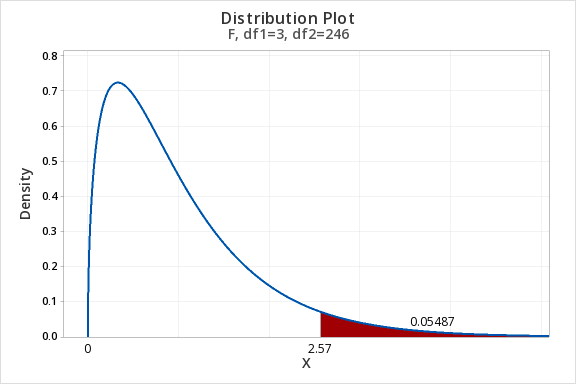
\includegraphics[width=1\textwidth]{images/F - pvalue.png}
    \caption{\en{F and p-value}}
\end{figure}

Ο υπολογισμός τώρα του \en{p-value} από το $F$ γίνεται μέσω της παραγωγής τυχαίων δεδομένων
και υπολογίζοντας το $F$ για αυτό το σετ. Αυτό γίνεται για αρκετές επαναλήψεις (όσο
περισσότερες τόσο το καλύτερο) και τα αποτελέσματα ($F$) που παίρνουμε τα τοποθετούμε σε
ένα ιστόγραμμα. Έπειτα βρίσκουμε το $F$ για το σετ δεδομένων που εξετάζουμε και το
τοποθετούμε και αυτό στο ιστόγραμμα.

Το \en{p-value} υπολογίζεται από τον αριθμό των τιμών
που είναι μεγαλύτερες από το $F$ του σετ που εξετάζουμε διαιρεμένο με τον αριθμό όλων των
τιμών. Στην πράξη το γράφημα του ιστογράμματος προσεγγίζεται από μία γραμμή $F$
κατανομής, έτσι ώστε να μην χρειαστεί να παράξουμε τόσο μεγάλο όγκο τυχαίων δεδομένων.
Το σχήμα της γραμμής εξαρτάται από τον αριθμό των δεδομένων και τους βαθμούς
ελευθερίας. Το \en{p-value} παίρνει μικρότερες τιμές όσο περισσότερα δείγματα έχουμε ανά
παράμετρο. Όσο μικρότερο το \en{p-value} τόσο καλύτερο το $R^2$
και κατά συνέπεια η γραμμή
παλινδρόμησης
\subsection{Πολλαπλή Παλινδρόμηση}
Η πολλαπλή παλινδρόμηση είναι παρόμοια με την απλή γραμμική μόνο που αντί να
εξετάζουμε την σχέση μεταξύ μίας ανεξάρτητης και μιας εξαρτημένης μεταβλητής,
εξετάζουμε την σχέση αυτή παίρνοντας υπόψιν πάνω από μία ανεξάρτητη (π.χ. για την
πρόβλεψη εκδήλωσης διαβήτη σε έναν ασθενή, λαμβάνουμε υπόψιν εκτός από το επίπεδο
ινσουλίνης στο αίμα του, το βάρος, την πίεση και άλλες βιολογικές μετρικές για τις οποίες
μπορεί να εξεταστεί). Ένα από τα μεγαλύτερα πλεονεκτήματα της πολλαπλής παλινδρόμησης
είναι ότι η μέθοδος ελαχίστων τετραγώνων που χρησιμοποιεί, από την φύση του απορρίπτει
ή μειώνει την επιρροή των μεταβλητών που δεν σχετίζονται ή δεν είναι τόσο καλές για το
μοντέλο.

Με αυτή την λογική δεν υπάρχει περίπτωση να χειροτερέψει ένα μοντέλο από την
πρόσθεση οποιασδήποτε μεταβλητής. Ωστόσο υπάρχουν δύο προβλήματα με αυτό. Το
πρώτο σχετίζεται με το κόστος σε χρόνο και πόρους που θα χρησιμοποιηθούν σε μία
μεταβλητή η οποία δεν θα βελτιώσει πολύ ή ενδεχόμενος και καθόλου το μοντέλο. Και το
δεύτερο είναι μια μεταβλητή που δεν σχετίζεται με το μοντέλο λόγω τυχαιότητας μπορεί να
αποδώσει λανθασμένα σε καλύτερη προσαρμογή της παλινδρόμησης.

Ο τρόπος
υπολογισμού της δεν διαφέρει από αυτόν της απλής γραμμικής, το μόνο που προσθέτουμε
είναι επιπλέον άξονες (διαστάσεις) στο μοντέλο. Αυτό προφανώς έχει αντίκτυπο στην μορφή
που θα έχει η παλινδρόμηση, όπου για δυο ανεξάρτητες μεταβλητές θα έχουμε ένα επίπεδο
αντί για ευθεία (2 διαστάσεις) και όσο περισσότερες μεταβλητές (διαστάσεις) προσθέτουμε
θα προσαρμόζεται ανάλογα και η παλινδρόμηση, χωρίς να χάνεται η γραμμικότητα της.

\begin{figure}[H]
    \centering
    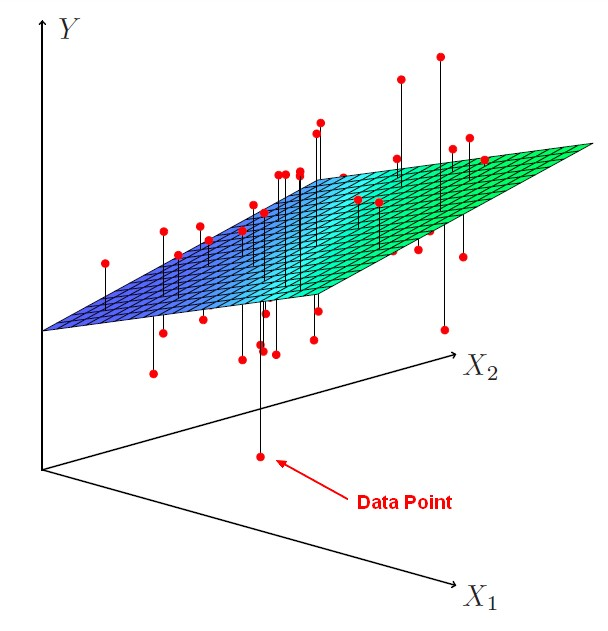
\includegraphics[width=1\textwidth]{images/Multiple regression.jpg}
    \caption{Πολλαπλή παλινδρόμηση}
\end{figure}

Μία άλλη
διαφορά είναι ότι σε αυτή την περίπτωση είναι αναγκαίο να χρησιμοποιήσουμε το
προσαρμοσμένο $R^2$ αντί για το $R^2$ με το πρώτο να είναι απλά μία παραλλαγή του δεύτερου
λαμβάνοντας υπόψιν και τις επιπλέον διαστάσεις στον υπολογισμό του. Το προσαρμοσμένο
$R^2$ δίνεται από την σχέση:
$$R_{\enm{adj}}=1-\frac{(1-R^2)(n-1)}{n-p-1}$$
όπου:
\begin{description}
    \item[$n$ :] το πλήθος των δειγμάτων
    \item[$p$ :] το πλήθος των ανεξάρτητων μεταβλητών (\en{regressors})
\end{description}
Το πλεονέκτημα με το προσαρμοσμένο $R^2$
είναι ότι μειώνει την αδυναμία του $R^2$
να
αυξάνεται με την πρόσθεση επιπλέον μεταβλητών που δεν προσαρμόζονται καλά στα
δεδομένα. Το προσαρμοσμένο $R^2$
λύνει αυτό το πρόβλημα \tqt{τιμωρώντας} το αποτέλεσμα
όταν προσθέτονται τέτοιες μεταβλητές που δεν είναι αρκετά καλές. Έτσι το προσαρμοσμένο $R^2$
θα είναι πάντα μικρότερο ή ίσο του $R^2$. Χρησιμοποιώντας το νέο προσαρμοσμένο $R^2$ στην
θέση του $R^2$ υπολογίζουμε το \en{p-value}.

Με τα παραπάνω συγκρίνουμε την παλινδρόμηση στην μέση τιμή. Το δυνατό σημείο της
πολλαπλής παλινδρόμησης ωστόσο είναι στην σύγκριση της απλής γραμμικής με μία
πολλαπλή ή μιας πολλαπλής με μία πολλαπλή με παραπάνω μεταβλητές. Η σύγκριση αυτή
είναι πολύ σημαντική, καθώς μας δείχνει το πόσο βελτιώνεται η πρόβλεψη μας εάν
προσθέσουμε την μεταβλητή (ή μεταβλητές) αυτή και το εάν αξίζει να αφιερώσουμε
πολύτιμο χρόνο και πόρους για τον υπολογισμό της.

Η σύγκριση αυτή μπορεί να γίνει είτε
συγκρίνοντας τα 2 προσαρμοσμένα $R^2$
και τα \en{p-values} τους ή (αυτό που προτείνεται) να
υπολογίσουμε εκ νέου τις μετρικές αυτές αλλά αντί για \en{mean} να βάλουμε τις τιμές του \en{simple}
(απλούστερου) μοντέλου και αντί για το \en{fit} να βάλουμε το ποιο πολύπλοκο (πολλαπλό) , έτσι
θα έχουμε:

$$R^2=\frac{\enm{Var}(\enm{simple})-\enm{Var}(\enm{complex})}{\enm{Var}(\enm{simple})}$$
\\
$$\mathlarger{F =\frac{\frac{\enm{SS}(\enm{simple}) - \enm{SS}(\enm{complex})}{p_{\enm{complex}} - p_{\enm{simple}}}} {\frac{\enm{SS}(\enm{complex})}{n - p_{\enm{complex}}}}}$$
Εάν το προσαρμοσμένο $R^2$
είναι μεγάλο και το \en{p-value} μικρό τότε αξίζει να υπολογίσουμε την
(τις) επιπλέον μεταβλητή.
\subsection{\en{T-test}}
Το τ-τεστ είναι ένα στατιστικό τεστ και χρησιμοποιείται κυρίως για την σύγκριση 2 ομάδων, στο
πεδίο των δοκιμών υποθέσεων (\en{hypothesis testing}), για να βρούμε τι επιρροή θα έχει η
αλλαγή ενός χαρακτηριστικού της ομάδας.

Για παράδειγμα ένα τέτοιο τεστ στον τομέα της
βιολογίας μπορεί να αφορούσε την αλλαγή ενός γονιδίου ή την χορήγηση ενός φαρμάκου
έχοντας ένα \en{control group} (χωρίς να παίρνει το φάρμακο ή \en{placebo}) και ένα που να
χορηγείται. Λόγο της ομαδοποίησης τους με τέτοιο τρόπο τα δεδομένα έχουν διακριτές τιμές
στον άξονα της ανεξάρτητης μεταβλητής (με ή χωρίς / ομάδα 1 ή ομάδα 2). Φυσικά στις δύο
ομάδες που ελέγχουμε, μπορούμε να χρησιμοποιήσουμε τεχνικές παλινδρόμησης για να
αναλύσουμε τις ομοιότητες και τις διαφορές των ομάδων και να χαρακτηρίσουμε την
επίδραση της αλλαγής. Για δείξουμε τον τρόπο εφαρμογής των τεχνικών θα αναλύσουμε ένα
παράδειγμα.

Έστω ότι έχουμε 2 ομάδες μία με το σύνηθες γονίδιο Α και μία με το ποιο σπάνιο
μεταλλαγμένο γονίδιο Β. Το γονίδιο αυτό (μεταλλαγμένο και μη) επηρεάζει την
εμφάνιση της στεφανιαίας νόσου που είναι μια πάθηση της καρδιάς (\en{heart disease}) και θέλουμε
να αναλύσουμε την επίδραση μου έχει το καθένα στην εκδήλωση της ασθενείας. Αρχικά
πρέπει να βρούμε ένα μέσο(\en{mean}) για όλα τα δείγματα (Α και Β) και να βρούμε τo \en{SSR(mean)}.
Αυτό το κάνουμε ακριβώς όπως στην απλή γραμμική.

Τώρα θα πρέπει να προσαρμόσουμε 2
γραμμές μία σε κάθε ομάδα. Μπορεί να αποδειχθεί ότι την καλύτερη προσαρμογή (\en{best fit})
με την μέθοδο των μικρότερου αθροίσματος τετραγώνων (\en{least squares fit}) θα έχει ο μέσος
όρος τους. Οι γραμμές που βρήκαμε θα είναι γραμμές παράλληλες στον άξονα $x$ και τα
τέμνουν το $y$ στην μέση τιμή των δεδομένων του κάθε γκρουπ. Τώρα πρέπει να βρούμε έναν
τρόπο να ενώσουμε τις δύο γραμμές σε μία συνάρτηση ώστε να μπορούμε να το περάσουμε
σε ένα υπολογιστικό σύστημα για να κάνει όλους τους δύσκολους υπολογισμούς (πχ
μετρικών $R^2$, \en{p-value}).

Για χάρη απλότητας θα έχουμε ένα πολύ μικρό δείγμα για να
εξηγήσουμε την τεχνική.
Έστω λοιπών ότι έχουμε 3 δείγματα από κάθε ομάδα (σύνολο 6) τότε η σχέση που υπολογίζει
και τις δύο γραμμές είναι η εξής:
\begin{gather*}
    y=1\times (\enm{\textbf{meanA}}) + 0\times (\enm{meanB}) + (\enm{residual\_1})\\
    y=1\times (\enm{\textbf{meanA}}) + 0\times (\enm{meanB}) + (\enm{residual\_2})\\
    y=1\times (\enm{\textbf{meanA}}) + 0\times (\enm{meanB}) + (\enm{residual\_3})\\
    \\
    y=0\times (\enm{meanA}) + 1\times (\enm{\textbf{meanB}}) + (\enm{residual\_4})\\
    y=0\times (\enm{meanA}) + 1\times (\enm{\textbf{meanB}}) + (\enm{residual\_5})\\
    y=0\times (\enm{meanA}) + 1\times (\enm{\textbf{meanB}}) + (\enm{residual\_6})
\end{gather*}

Παρατηρούμε πως η σχέση είναι ίδια για όλα τα δείγματα, το μόνο που αλλάζει είναι οι
συντελεστές μπροστά από τα 2 \en{mean} οι οποίοι μάλιστα παίρνουν τιμές 1 και 0. Οι
συντελεστές που μόλις αναφέραμε λειτουργούν σαν διακόπτες για το ποια ομάδα
διαλέγουμε. Τους συντελεστές μπορούμε να τους έχουμε σε έναν πίνακα που ονομάζεται
\en{design matrix}. Με την παραλλαγή αυτή η σχέση μετατρέπεται σε:
$$y=\enm{column1}\times \enm{meanA} + \enm{column2}\times \enm{meanB}$$
Όπου:
\begin{table}[H]
    \centering
    \begin{tabular}{|c|c|}
        \hline
        \en{column1} & \en{column2} \\ \hline
        1 & 0 \\ \hline
        1 & 0 \\ \hline
        1 & 0 \\ \hline
        0 & 1 \\ \hline
        0 & 1 \\ \hline
        0 & 1 \\ \hline
    \end{tabular}
\end{table}
Αφού έχουμε τον τύπο και για τις 2 γραμμές βρίσκουμε το \en{SSR(fit)} για κάθε ομάδα (απόσταση
δείγματος και γραμμής ομάδας). Έχοντας και το \en{SSR(fit)} μπορούμε να υπολογίσουμε το $R^2$
και το \en{p-value} για τις 2 γραμμές παλινδρόμησης.
Σε αυτό το σημείο θα αλλάξουμε λίγο την σχέση σε μία που χρησιμοποιείται πιο συχνά,
ωστόσο και οι δύο βγάζουν το ίδιο σωστό αποτέλεσμα. Η νέα σχέση θα είναι:
$$y=\enm{column1}\times \enm{meanA} + \enm{column2}\times \enm{difference}(\enm{meanB}-\enm{meanA})$$
Και το \en{design matrix} θα γίνει:
\begin{table}[H]
    \centering
    \begin{tabular}{|c|c|}
        \hline
        \en{column1} & \en{column2} \\ \hline
        1 & 0 \\ \hline
        1 & 0 \\ \hline
        1 & 0 \\ \hline
        1 & 1 \\ \hline
        1 & 1 \\ \hline
        1 & 1 \\ \hline
    \end{tabular}
\end{table}
Με λίγα λόγια η νέα σχέση υπολογίζει και τις δύο γραμμές, αλλά τώρα η δεύτερη είναι σε
μορφή \en{offset} από την πρώτη. Τέτοιου είδους \en{design matrix} μπορεί να χρησιμοποιηθεί και για
απλή γραμμική παλινδρόμηση με την μόνη διαφορά ότι αντί για διακριτές τιμές μπορούμε
να έχουμε οποιαδήποτε τιμή θέλουμε κρατώντας την πρώτη στήλη στο 1 για το \en{intercept}.

Τώρα που ξέρουμε τι είναι και από τι αποτελείται ένα \en{t-test} θα τα αναμείξουμε με τις τεχνικές
της παλινδρόμησης που αναφέραμε πιο πάνω για αναλύσουμε το \en{t-test} και για να βγάλουμε
κάποια χρήσιμα συμπεράσματα. Για να δείξουμε πως ενώνουμε τα \en{t-test} με την
παλινδρόμηση θα χρησιμοποιήσουμε το παράδειγμα που είχαμε παραπάνω με τα δύο
γονίδια Α(κόκκινο) και Β(πράσινο) με τον άξονα $y$ να είναι η πιθανότητα να εμφανιστεί η
νόσος και το $x$ να είναι η ηλικία.

\begin{figure}[H]
    \centering
    \begin{tikzpicture}
        \begin{axis}[xmin = 0, xmax=5, ymin=0, ymax=5, xtick=\empty, ytick=\empty, axis lines=left, scatter/classes={
            a={mark=o,red},
            b={mark=o,green}
        }]
            \addplot[scatter, only marks, scatter src=explicit symbolic] coordinates {
                (1,1.1) [a]
                (2,1.8) [a]
                (3,3.2) [a]
                (4,3.7) [a]
                (1.5,1.3) [a]
                (2.5,2.3) [a]
                (3.5,3.7) [a]
                (4.5,4.6) [a]
                (5,5) [a]

                (0.5,2.3) [b]
                (1,3.1) [b]
                (2,3.8) [b]
                (3,5.2) [b]
                (4,5.7) [b]
                (1.5,3.7) [b]
                (2.5,4.6) [b]
                (3.2,5) [b]
            };
        \end{axis}
    \end{tikzpicture}
    \caption{\en{T-test}}
\end{figure}

Βλέπουμε πως τα άτομα με το Β γονίδιο έχουν μεγαλύτερη πιθανότητα να εμφανίσουν την
νόσο από τα άτομα με το Α γονίδιο και βλέπουμε ότι οι δύο ομάδες ακολουθούν δύο
διαφορετικές παλινδρομήσεις.

\begin{figure}[H]
    \centering
    \begin{tikzpicture}
        \begin{axis}[xmin = 0, xmax=5, ymin=0, ymax=5, xtick=\empty, ytick=\empty, axis lines=left, scatter/classes={
            a={mark=o,red},
            b={mark=o,green}
        }]
            \addplot[scatter, only marks, scatter src=explicit symbolic] coordinates {
                (1,1.1) [a]
                (2,1.8) [a]
                (3,3.2) [a]
                (4,3.7) [a]
                (1.5,1.3) [a]
                (2.5,2.3) [a]
                (3.5,3.7) [a]
                (4.5,4.6) [a]
                (5,5) [a]

                (0.5,2.3) [b]
                (1,3.1) [b]
                (2,3.8) [b]
                (3,5.2) [b]
                (4,5.7) [b]
                (1.5,3.7) [b]
                (2.5,4.6) [b]
                (3.2,5) [b]
            };
            \addplot[dashed, blue] {x+2};
            \addplot[dashed, orange] {x};
        \end{axis}
    \end{tikzpicture}
    \caption{Συνδυασμός παλινδρόμησης με \en{T-test}}
\end{figure}

Εάν κάναμε μία παλινδρόμηση στο σύνολο των δειγμάτων θα βγάζαμε μία γραμμή που θα
περνούσε ανάμεσα από τις 2 γραμμές που βλέπουμε και θα είχε πολύ μεγάλη διακύμανση
κάτι που είναι εντελώς λάθος να κάνουμε. Επίσης ένα απλό \en{t-test} δεν θα λάμβανε υπόψιν την
συσχέτιση της ηλικίας με την πιθανότητα εμφάνισης της νόσου και η παλινδρόμηση όπως
είδαμε δεν θα λάμβανε υπόψιν την διαφορά στο γονίδιο.

Έτσι για τον συνδυασμό τους θα
έχουμε 2 διαφορετικές παλινδρομήσεις μία για κάθε ομάδα και θα τις συγκρίνουμε μεταξύ
τους, κάτι που θα έκανε ένα απλό \en{t-test} στα 2 \en{mean}. Για να κάνουμε απλά τα πράγματα στο
συγκεκριμένο παράδειγμα οι δύο παλινδρομήσεις έχουν την ίδια κλίση και η μόνη διαφορά
τους είναι το σημείο τομής με τον $y$ άξονα.

Στην πραγματικότητα θα μπορούσαμε να έχουμε
και διαφορετικές κλίσεις προσθέτοντας στον τύπο που θα δώσουμε παρακάτω μερικές
επιπλέον μεταβλητές και στο \en{Design matrix} μερικές στήλες για τις αντίστοιχες μεταβλητές.
Έτσι λοιπόν θα έχουμε:
$$y=\enm{column1}\times \enm{intersectA} + \enm{column2}\times \enm{intersect\_offset} + \enm{column3}\times \enm{slope}$$
Και το \en{design matrix} θα γίνει:
\begin{table}[H]
    \centering
    \begin{tabular}{|c|c|c|}
        \hline
        \en{column1} & \en{column2} & \en{column3} \\ \hline
        1 & 0 & $X(1)$ \\ \hline
        1 & 0 & $X(2)$ \\ \hline
        1 & 0 & $X(3)$ \\ \hline
        1 & 1 & $X(4)$ \\ \hline
        1 & 1 & $X(5)$ \\ \hline
        1 & 1 & $X(6)$ \\ \hline
    \end{tabular}
\end{table}
Υπολογίζοντας τις αποστάσεις από την γραμμή παλινδρόμησης (\en{residual}) για την κάθε ομάδα
ξεχωριστά (Β γονίδιο από την μπλε γραμμή και Α αντίστοιχα από την πορτοκαλί) μπορούμε
να βρούμε το $R^2$
και το \en{p-value} για το μοντέλο χρησιμοποιώντας το απλό μοντέλο του μέσου
όρου όλων των τιμών ή να το συγκρίνουμε με οποιαδήποτε άλλο μοντέλο μέσω των
παρακάτω τύπων.

Το δεύτερο γίνεται για να δούμε εάν κάποια μεταβλητή ό ομαδοποίηση
είναι χρήσιμη για το μοντέλο και αν αξίζει να την υπολογίσουμε:
$$R^2=\frac{\enm{Var}(\enm{simple})-\enm{Var}(\enm{complex})}{\enm{Var}(\enm{simple})}$$
\\
$$\mathlarger{F =\frac{\frac{\enm{SS}(\enm{simple}) - \enm{SS}(\enm{complex})}{p_{\enm{complex}} - p_{\enm{simple}}}} {\frac{\enm{SS}(\enm{complex})}{n - p_{\enm{complex}}}}}$$


Επίσης υπάρχουν και τα \en{ANOVA} τα οποία είναι σαν τα τ-τεστ αλλά με περισσότερες ομάδες, πχ για το προηγούμενο
παράδειγμα θα μπορούσαμε να έχουμε το γονίδιο Α και Β σε κανονική διατροφή. Παράλληλα θα έχουμε άλλες ομάδες
των 2 γονιδίων αλλά να είναι μέσα σε ειδικό πρόγραμμα διατροφής ή να έχουν κάποια
φαρμακευτική αγωγή που θέλουμε να ελέγξουμε και να έχουμε 2 \en{control groups}( A και B), 2
\en{placebo} και 2 που θα παίρνουν την αγωγή. Ο υπολογισμός τέτοιων μοντέλων είναι ο ίδιος με
τα \en{t-test} μόνο που για συνολική γραμμή υπολογίζουμε τις παλινδρομήσεις όλων των ομάδων
και για $p_{fit}$ για τον υπολογισμού του $F$ θα βάλουμε τον αντίστοιχο αριθμό των ομάδων.
\subsection{Πολυωνυμική Παλινδρόμηση}
Η πολυωνυμική παλινδρόμηση είναι η γενικότερη κατηγορία παλινδρόμησης στην οποία
ανήκουν τα διάφορα είδη της γραμμικής παλινδρόμησης που είδαμε προηγουμένως και κατά
ακολουθία ανήκει στα τυπικά γραμμικά μοντέλα (\en{Standard Linear Models}).

Η ειδοποιός
διαφορά που μας κάνει να τα ξεχωρίζουμε σαν δύο διαφορετικές κατηγορίες είναι το γεγονός
ότι αντί η γραμμή παλινδρόμησης να χαρακτηρίζεται από μία ευθεία γραμμή μπορεί να έχει
και μία κυρτότητα ώστε να \tqt{ακολουθάει} καλύτερα τα δεδομένα, όπου με την σειρά τους δεν
έχουν γραμμική εξάρτηση από την ή τις ανεξάρτητες μεταβλητές. Η γραμμή πολυωνυμικής
παλινδρόμησης δίνεται από τον τύπο:
$$y_i=a_0+a_1x_i+a_2x_i^2+\cdots +a_nx_i^n+\epsilon$$
Πολύ εύκολα μπορούμε να δούμε ότι η απλή γραμμική παλινδρόμηση είναι μία πολυωνυμική
1\textsuperscript{ου} βαθμού. Ο βαθμός (τάξη) του πολυωνύμου όπως ξέρουμε είναι η μεγαλύτερη δύναμη
στην οποία υψώνεται η (ανεξάρτητη) μεταβλητή.

Θα ρωτούσε κανείς πώς γίνεται να είναι η
γενικότερη κατηγορία όλων των γραμμικών παλινδρομήσεων όταν υπάρχουν όροι υψωμένοι
σε δύναμη μεγαλύτερη του 1. Η απάντηση σε αυτό το ερώτημα θα ήταν ότι παρόλο που οι
ανεξάρτητες μεταβλητές είναι μη γραμμικές, οι συντελεστές είναι, και αποκλειστικά
τα δεδομένα είναι αυτά που υψώνονται σε μεγαλύτερες δυνάμεις.

Ο τρόπος υπολογισμού των συντελεστών γίνεται με χρήση πινάκων, για αυτό και θα πρέπει
να αναπαραστήσουμε την πολυωνυμική παλινδρόμηση σε μορφή πινάκων ως εξής:
$$
\begin{bmatrix}
    y_1  \\
    y_2 \\
    \vdots \\
    y_n
\end{bmatrix}
=
\begin{bmatrix}
    1       & x_1    & \dots     & x_1^m \\
    1       & x_2    & \dots     & x_2^m \\
    \vdots  & \vdots    & \ddots    & \vdots \\
    1       & x_n    & \dots     & x_n^m \\
\end{bmatrix}
\times
\begin{bmatrix}
    a_0 \\
    a_1 \\
    \vdots \\
    a_k
\end{bmatrix}
+
\begin{bmatrix}
    \epsilon_0 \\
    \epsilon_1 \\
    \vdots \\
    \epsilon_k
\end{bmatrix}
$$
Όπου απλοποιείται σε:
$$\overrightarrow{y}=X\overrightarrow{a}+\overrightarrow{\epsilon}$$
Επομένως με την χρήση της μεθόδου ελαχίστων τετραγώνων έχουμε:
$$\widehat{\overrightarrow{b}}=(X^TX)^{-1}X^T\overrightarrow{y}$$
Ή ένας εναλλακτικός τρόπος είναι να λύσουμε το παρακάτω σύστημα:
$$
\begin{bmatrix}
    N       & \sum\limits_{i=1}^Nx_i    & \dots     & \sum\limits_{i=1}^Nx_i^k \\
    \sum\limits_{i=1}^Nx_i   & \sum\limits_{i=1}^Nx_i^2       & \dots     & \sum\limits_{i=1}^Nx_i^{k+1} \\
    \vdots  & \vdots    & \ddots    & \vdots \\
    \sum\limits_{i=1}^Nx_i^k   & \sum\limits_{i=1}^Nx_i^{k+1}    & \dots     & \sum\limits_{i=1}^Nx_i^{2k}
\end{bmatrix}
\times
\begin{bmatrix}
    a_0 \\
    a_1 \\
    \vdots \\
    a_k
\end{bmatrix}
=
\begin{bmatrix}
    \sum\limits_{i=1}^Ny_i  \\
    \sum\limits_{i=1}^Nx_iy_i \\
    \vdots \\
    \sum\limits_{i=1}^Nx_i^ky_i
\end{bmatrix}
$$
Έπειτα χρησιμοποιώντας την μέθοδο του \en{Cramer} βρίσκουμε τους συντελεστές ως εξής:
$$a_k=\frac{\det (M_i)}{\det (M)}$$
\\
$$
M_0=
\begin{bmatrix}
    \sum\limits_{i=1}^Ny_i          & \sum\limits_{i=1}^Nx_i        & \dots     & \sum\limits_{i=1}^Nx_i^k \\
    \sum\limits_{i=1}^Nx_iy_i          & \sum\limits_{i=1}^Nx_i^2      & \dots     & \sum\limits_{i=1}^Nx_i^{k+1} \\
    \vdots                          & \vdots                        & \ddots    & \vdots \\
    \sum\limits_{i=1}^Nx_i^ky_i        & \sum\limits_{i=1}^Nx_i^{k+1}  & \dots     & \sum\limits_{i=1}^Nx_i^{2k}
\end{bmatrix}
$$
Ενώ έχοντας πλέον την πολυωνυμική παλινδρόμηση με τους συντελεστές της ο τρόπος
υπολογισμού του \en{SSR} παραμένει ίδιος. Εφόσον έχουμε το \en{SSR} μπορούμε να εφαρμόσουμε
όλα όσα αναφέραμε και στην απλή γραμμική παλινδρόμηση.

Επίσης όσο μεγαλύτερη η τάξη του πολυωνύμου, τόσο πιο \tqt{στενά} θα προσαρμόζεται η
παλινδρόμηση στα δεδομένα. Αναφερόμενοι στις δυνάμεις, ο μόνος περιορισμός που
υπάρχει για το μέγιστο βαθμό που πολυωνύμου είναι ότι δεν πρέπει να ξεπερνάει τον αριθμό
των δεδομένων, γεγονός που δεν θα μας επιτρέπει να προσαρμόσουμε την ευθεία στα
δεδομένα. Κάτι τέτοιο προφανώς (η τάξη να πλησιάσει τον αριθμό των δεδομένων) σπανίως
είναι επιθυμητό, εάν όχι καθόλου, καθώς είναι σχεδόν σίγουρο ότι θα οδηγήσει σε \en{over-fitting}.

Πως υπολογίζουμε την κατάλληλη τάξη του πολυωνύμου?


\begin{figure}[H]
    \centering
\begin{subfigure}{1\textwidth}
    \centering
    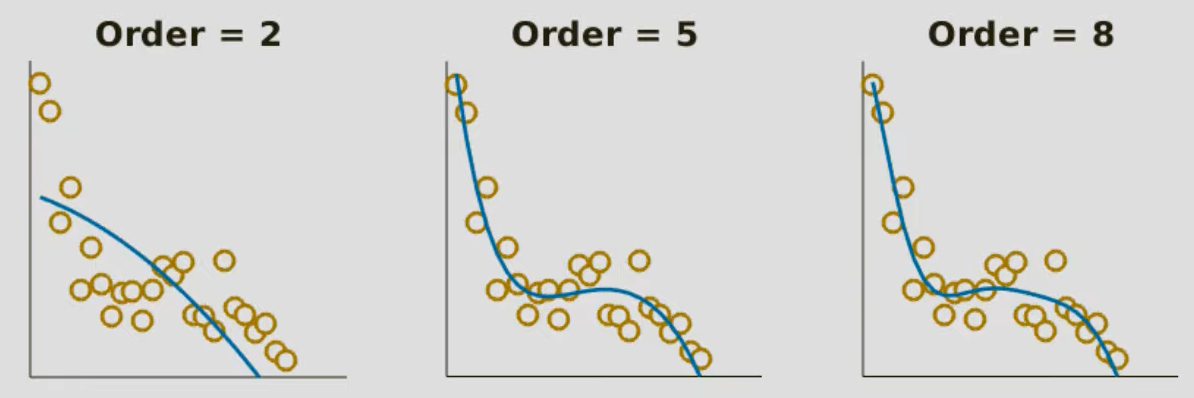
\includegraphics[width=1\textwidth]{images/Polynomial order 2_1.png}
\end{subfigure}
\begin{subfigure}{1\textwidth}
    \centering
    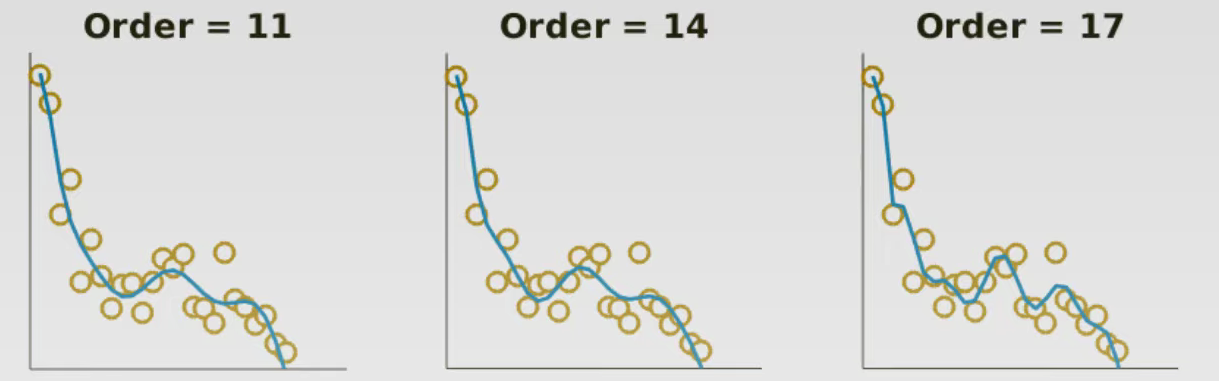
\includegraphics[width=1\textwidth]{images/Polynomial order 2_2.png}
\end{subfigure}
\caption{Τάξη πολυωνυμικής παλινδρόμησης}
\end{figure}

Το πρόβλημα της εύρεσης κατάλληλου βαθμού για το πολυώνυμο το λύνει το \en{Bayes Information Criteria (BIC)}:
$$\enm{BIC}_k=n\log (\enm{SSR})+K\log (n)$$
Όπου:
\begin{description}
    \item[$k$ :] βαθμός πολυωνύμου
    \item[$n$ :] βαθμός αριθμός δεδομένων
\end{description}
Η ποσότητα αυτή υπολογίζεται για κάθε βαθμό του πολυωνύμου και επιλέγεται η μικρότερη
ως η καλύτερη για το εκάστοτε μοντέλο. Αν αναπαραστήσουμε τις ποσότητες που
βρήκαμε, για ένα μοντέλο όπου τα δεδομένα ακολουθούν μία συνάρτηση 3\textsuperscript{ου} βαθμού
παρατηρούμε ότι ο υπολογισμός της βέλτιστης τάξης είναι σωστός.

\begin{figure}[H]
    \centering
    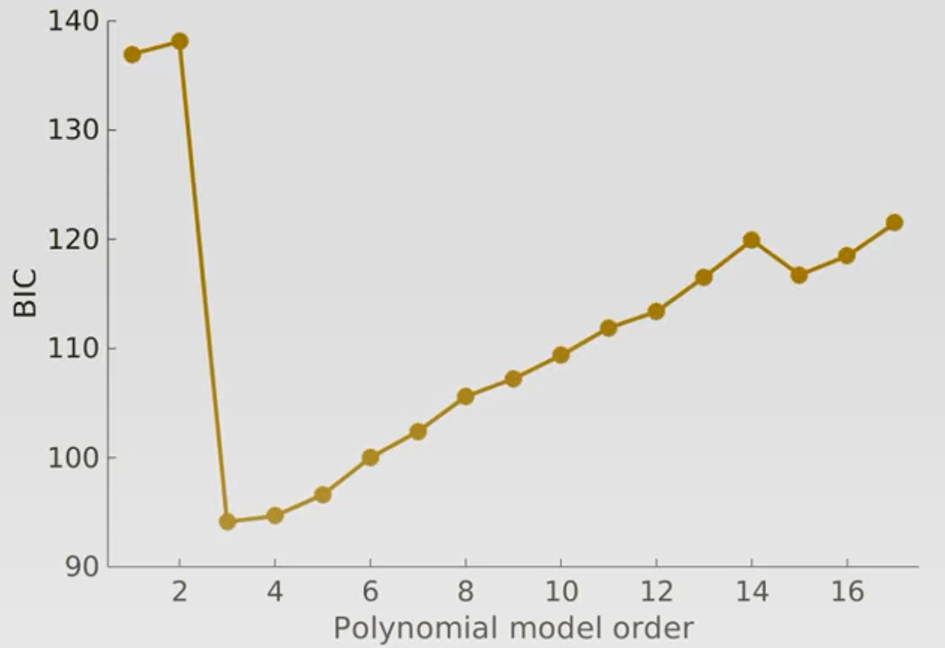
\includegraphics[width=1\textwidth]{images/BIC_2.png}
    \caption{Βέλτιστη τάξη}
\end{figure}
\subsection{Λογαριθμική Παλινδρόμηση}
Η λογαριθμική παλινδρόμηση δουλεύει με συνεχής μεταβλητές  όπως το βάρος αλλά και διακριτές
όπως το φύλλο. Σαν έξοδο παρέχει μία
\en{Boolean} τιμή (\en{true, false} ή έχει/δεν έχει κάποια ασθένεια) προδίδοντας παράλληλα και μία
πιθανότητα (σωστής) πρόβλεψης. Παρατηρώντας κάποιος αυτή την ιδιότητα καταλαβαίνει
ότι είναι πολύ χρήσιμη σε εφαρμογές ταξινόμησης όπου και χρησιμοποιείται κατά κύριο
λόγο.

Η ικανότητα αυτή για ταξινόμηση την κάνει ευρέως γνωστή τον τομέα της μηχανικής
μάθησης. Για παράδειγμα χρησιμοποιώντας αυτού του είδους την παλινδρόμηση θα
μπορούσαμε να προβλέψουμε με τα αποτελέσματα κάποιων αιματολογικών εξετάσεων και
γνωρίζοντας την ηλικία και το φύλο του εξεταζόμενου εάν πάσχει από κάποια ασθένεια και
ποια είναι η πιθανότητα, αυτή η πρόβλεψη να είναι ακριβής.

Μια διαφορά με την
γραμμική παλινδρόμηση είναι ο τρόπος που προσαρμόζουμε την παλινδρόμηση στα
δεδομένα. Στην λογαριθμική επειδή η παλινδρόμηση έχει μία σιγμοειδή μορφή δεν
μπορούμε να χρησιμοποιήσουμε την μέθοδο ελαχίστων τετραγώνων, αλλά χρησιμοποιείται
η μέθοδος της μέγιστης πιθανότητας (\en{maximum likelihood}).

Κάτι που δεν αναφέρθηκε πριν για την απλή γραμμική παλινδρόμηση είναι ότι δεν έχει
φραγμένα όρια για τις μεταβλητές τις κάτι που την κάνει πιο εύκολη στον υπολογισμό αλλά
και επιρρεπή σε λάθη ως προς την φυσική ορθότητα του μοντέλου. Για παράδειγμα εάν
είχαμε ένα μοντέλο όπου θα συσχετίζαμε ορθά το μέγεθος (όγκο) ενός ζώου ή ανθρώπου με
το βάρος του, όπου ζώα με μεγαλύτερο βάρος θα είχαν και μεγαλύτερο μέγεθος, μπορούμε
να υπολογίσουμε το μέγεθος ζώου με μηδενικό ή και αρνητικό βάρος, κάτι που προφανώς
δεν είναι δυνατόν να γίνει στον φυσικό κόσμο. Αντίθετα στην λογαριθμική παλινδρόμηση δεν
γίνεται κάτι τέτοιο και ο άξονας της εξαρτημένης μεταβλητής είναι φραγμένος στο πεδίο $[0,1]$.
Για να λύσουμε αυτό το θέμα μετατρέπουμε την πιθανότητα (του άξονα $y$) σε λογάριθμο της
πιθανότητας ώστε ο άξονας να παίρνει τιμές από $-\infty$ ως $\infty$. Η μετατροπή αυτή γίνεται με
την συνάρτηση \en{logit} που ορίζεται από τον τύπο:
$$\log(\enm{odds})=\log\left(\frac{p}{1-p}\right)$$
Όπου:
\begin{description}
    \item[$p$ :] Η πιθανότητα του παλιού άξονα της εξαρτημένης μεταβλητής
\end{description}
\begin{gather*}
    \lim\limits_{p\rightarrow0}\left[\log\left(\frac{p}{1-p}\right)\right]=-\infty \\
    \log\left(\frac{0.5}{1-0.5}\right)=0\\
    \lim\limits_{p\rightarrow1}\left[\log\left(\frac{p}{1-p}\right)\right]=+\infty
\end{gather*}

\begin{figure}[H]
    \centering
    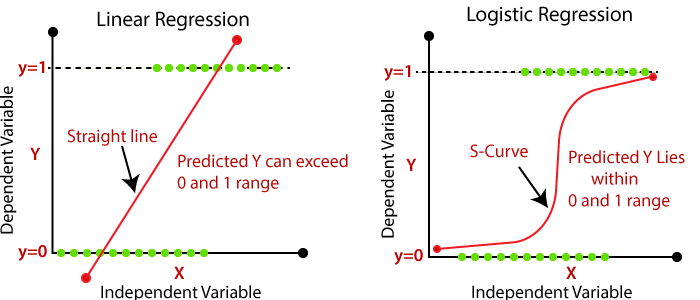
\includegraphics[width=1\textwidth]{images/linear-regression-vs-logistic-regression.png}
    \caption{Γραμμική και λογαριθμική παλινδρόμηση}
\end{figure}

Όλες οι άλλες ενδιάμεσες τιμές υπολογίζονται αντίστοιχα. Το αποτέλεσμα του
μετασχηματισμού είναι από την κυρτή (σιγμοειδή) γραμμή που είχαμε πριν, να έχουμε μία
ευθεία γραμμή χωρίς φραγμένο πεδίο ορισμού.

Τώρα ενώ τα δεδομένα και η λογαριθμική
παλινδρόμηση σχετίζονται και παρουσιάζονται στην προηγούμενη μορφή (γράφημα
πιθανοτήτων) όλες οι πράξεις και αναπαραστήσεις των συντελεστών θα γίνεται στο
μετασχηματισμένο μοντέλο (λογάριθμοι πιθανοτήτων). Έχοντας τώρα ένα γραμμικό μοντέλο
για τους συντελεστές μπορούμε να εφαρμόσουμε όλους τους υπολογισμούς και να
υπολογίσουμε τις μετρικές που είχαμε στην απλή γραμμική παλινδρόμηση με κάποιες
αλλαγές. Στη λογαριθμική παλινδρόμηση χρησιμοποιείται το \en{z-value} ή \en{Wald's test} που δίνεται από τον τύπο:
$$\enm{z-value}=\frac{\text{εκτίμιση}}{\text{τυπικό σφάλμα}}$$
και μας δείχνει πόσα τυπικά σφάλματα μακριά από το 0 είναι η εκτίμησή μας.

Όλα αυτά αφορούν τις συνεχές μεταβλητές. Για διακριτές μεταβλητές θα δουλέψουμε
περίπου με τον ίδιο τρόπο που δουλέψαμε στα \en{t-test} αλλά πρώτα πρέπει να κάνουμε την
μετατροπή του άξονα και μετά προσαρμόζουμε 2 γραμμές. Για παράδειγμα έστω ότι είχαμε να
μελετήσουμε την παλινδρόμηση για το πόσο μία μετάλλαξη σε ένα γονίδιο επηρεάζει την
πιθανότητα να αποκτήσει κάποιος διαβήτη. Για να βρούμε την γραμμή παλινδρόμησης για τα
άτομα που δεν έχουν την μετάλλαξη, θα πάρουμε τα άτομα αυτά και θα υπολογίσουμε την
τιμή του λογαρίθμου της πιθανότητας να έχουν διαβήτη (λογάριθμος πιθανότητας κανονικό):
$$\log\left(\frac{\text{άτομα με διαβήτη}}{\text{άτομα χωρίς διαβήτη}}\right)$$
Μετά θα υπολογίσουμε την ίδια τιμή (λογάριθμος πιθανότητας μετάλλαξης) και για τα άτομα
με την μετάλλαξη. Αυτές οι δύο τιμές θα είναι οι οριζόντιες γραμμές που είχαμε και στα \en{t-test}
και \en{ANOVA}. Για να δημιουργήσουμε την γραμμή της παλινδρόμησης θα συνδυάσουμε τις δύο
τιμές σε μία εξίσωση όπου τα $x$ είναι οι συντελεστές της:
$$y=\log(\text{πιθανότητα κανονικό})x_1 + \log\left(\frac{\text{πιθανότητα μετάλλαξης}}{\text{πιθανότητα κανονικό}}\right)x_2$$
Ο πρώτος όρος είναι το σημείο τομής και ο δεύτερος όρος μας λέει σε λογαριθμική κλίμακα πως
επηρεάζει το γονίδιο την πιθανότητα να έχεις διαβήτη.

Ο υπολογισμός της ευθείας έχει γίνει ποιο γρήγορος και εύκολος λόγω του μετασχηματισμού,
ωστόσο έχει δημιουργηθεί ένα πρόβλημα στον τρόπο προσαρμογής της στα δεδομένα,
καθώς τα δεδομένα αυτά έχουν πάρει τιμές $-\infty$ και $\infty$ για τα αντίστοιχα 0 και 1. Αυτό θέτει
αδύνατο τον υπολογισμό των ελάχιστο τετραγώνων αφού για όλα τα δεδομένα η απόσταση
από την ευθεία θα είναι $\infty$. Για αυτό όπως αναφέρθηκε πιο πάνω αντί για την μέθοδο των
ελάχιστων τετραγώνων χρησιμοποιείται η μέθοδος της μέγιστης πιθανότητας. Η μέθοδος
αυτή λειτουργεί προβάλλοντας τα δεδομένα στην εκάστοτε ευθεία που εξετάζουμε, σύμφωνα
με την θέση τους στον άξονα $x$, δίνοντάς τα μία τιμή λογαρίθμου πιθανότητας (άξονας $y$).
Έπειτα μετατρέπουμε αυτές τις τιμές λογαρίθμου πιθανότητας σε πιθανότητες μέσω του
αντίστροφου μετασχηματισμού που δίνεται από τον τύπο:
$$p=\frac{\mathlarger{e^{\log(\text{πιθανότητα})}}}{1+\mathlarger{e^{\log(\text{πιθανότητα})}}}$$

Τώρα που είμαστε στο αρχικό μοντέλο με την λογαριθμική παλινδρόμηση (φραγμένες τιμές
από 0 ως 1) και χρησιμοποιώντας τις πιθανότητες που βρήκαμε και την γνωστή κατάσταση
των δειγμάτων (πχ έχει ή δεν έχει διαβήτη) μπορούμε να υπολογίσουμε την μέγιστη
πιθανότητα. Αρχίζοντας με τα άτομα πού έχουν κατάσταση 1 (έχει διαβήτη) η πιθανότητα του
να έχει διαβήτη (να είναι στην κατάσταση 1) σύμφωνα με την παλινδρόμηση που εξετάζουμε
είναι η τιμή του άξονα $y$ για το συγκεκριμένο σημείο. Αντίστοιχα μετράμε και την πιθανότητα
να μην έχουν διαβήτη για τα άτομα που δεν έχουν διαβήτη (πιθανότητα τα άτομα που είναι
στην κατάσταση 0 να είναι σε αυτή την κατάσταση). Έτσι η πιθανότητα του μοντέλου δίνεται
από το γινόμενο των πιθανοτήτων αυτών:
$$\prod\limits_{i=1}^np_i\times\prod\limits_{i=1}^k(1-p_i)$$
Όπου:
\begin{description}
    \item[$n$ :] αριθμός ατόμων στην κατάσταση 1
    \item[$k$ :] αριθμός ατόμων στην κατάσταση 0
\end{description}

Πολλοί υπολογίζουν τον λογάριθμο αυτής της ποσότητας όπου απλά αντί να
πολλαπλασιάζεις τις πιθανότητες προσθέτεις τους λογαρίθμους των πιθανοτήτων ωστόσο
και τα δύο είναι ορθά αφού η ευθεία που μεγιστοποιεί τις πιθανότητες μεγιστοποιεί και τους
λογαρίθμους αυτωνών στο αντίστοιχο μετασχηματισμένο μοντέλο.
$$\sum\limits_{i=1}^n\log p_i+\sum\limits_{i=1}^k\log(1-p_i)$$

Για να βρεθεί η καλύτερη ευθεία με την βοήθεια ενός υπολογιστικού συστήματος
δοκιμάζουμε επαναληπτικά με \tqt{έξυπνους} αλγορίθμους που σε κάθε επανάληψη
βελτιώνουν την ευθεία (πχ γενετικοί αλγόριθμοι) πολλές τέτοιες ευθείες και απεικονίζουμε
τις πιθανότητες των μοντέλων (ευθειών). Η ευθεία με την μέγιστη πιθανότητα είναι η
καλύτερα προσαρμοσμένη.

Αφού βρήκαμε την ευθεία που προσαρμόζεται στα δεδομένα μας, το επόμενο βήμα (όπως
κάναμε και στην απλή γραμμική παλινδρόμηση) είναι να ελέγξουμε πόσο καλή είναι η
μεταβλητή που χρησιμοποιούμε βρίσκοντας το $R^2$
και το \en{p-value}. Ενώ στην απλή γραμμική ο
τρόπος για να βρούμε το $R^2$
είναι ένας και μοναδικός για την λογαριθμική παλινδρόμηση τα
πράγματα δεν είναι τόσο ξεκάθαρα. Υπάρχουν πάνω από 10 μέθοδοι εύρεσης του $R^2$
για την
λογαριθμική παλινδρόμηση. Εδώ θα εξετάσουμε μόνο έναν από αυτούς

Αρχικά στην θέση του \en{SSR} θα υπολογίζουμε το \en{LL} ($\log(\enm{likelihood}$) ) λογάριθμος πιθανότητας.
Για την τιμή \en{LL} της ευθείας που προσαρμόζεται (\en{fit}) ακολουθάμε την παραπάνω μεθοδολογία.
Για την μέση (\en{mean}) βρίσκουμε τον λογάριθμο της ολικής πιθανότητας να είναι σε κατάσταση
1, δηλαδή:
$$\log\left(\frac{n}{k}\right)$$

Αυτό μας δίνει μία τιμή, η οποία θα είναι το σημείο τομής του άξονα της εξαρτημένης
μεταβλητής και μίας ευθείας παράλληλη στον άξονα της ανεξάρτητης. Προβάλλοντας τα
δεδομένα σε αυτή την γραμμή και κάνοντας τον αντίστροφο μετασχηματισμό \en{logit}. Ένας
άλλος τρόπος να φτάσουμε στο ίδιο αποτέλεσμα είναι να βρούμε απευθείας την ολική
πιθανότητα να βρίσκεται κάποιος στην κατάσταση 1:
$$\frac{n}{n+k}$$

Αυτό μας δίνει έναν τρόπο να επαληθεύουμε τα αποτελέσματά μας. Για να τελειώσουμε την
διαδικασία αυτή πρέπει να βρούμε τον ολικό λογάριθμο πιθανότητας, ακολουθώντας τα
βήματα που δείξαμε παραπάνω για να βρούμε το $\enm{LL}(\enm{mean})$. Για το τελευταίο βήμα της
εύρεσης του $R^2$
κάνουμε μια παραλλαγή στον τύπο της απλής γραμμικής:
$$R^2=\frac{\enm{LL}(\enm{mean})-\enm{LL}(\enm{fit})}{\enm{LL}(\enm{mean})}$$
Κάνοντας το απλό πείραμα του να βάλουμε τιμές οι οποίες είναι εντελώς τυχαίες και η
μεταβλητή που εξετάζουμε δεν έχει καμία εξάρτηση από την ανεξάρτητη και υπολογίσουμε
το $R^2$, θα δούμε ότι παίρνει τιμή 0. Αντίστοιχα για έναν τέλειο προβλεπτή (\en{predictor}) θα
βρίσκαμε $R^2=1$. Άρα το $R^2$ ορθά είναι φραγμένο ανάμεσα στο 0 και το 1.

Για να βρούμε το \en{p-value} έχουμε τον εξής τύπο:
$$\chi^2=2(\enm{fit})-\enm{LL}(\enm{mean})$$
Όπου $\chi^2$ είναι μία τιμή με:
$$\text{Βαθμοί ελευθερίας}=\text{Βαθμοί ελευθερίας}(\enm{fit})-\text{Βαθμοί ελευθερίας}(\enm{mean})$$

Για μία απλή λογαριθμική παλινδρόμηση ο βαθμός ελευθερίας είναι $2 - 1 = 1$ και αυτό
βγαίνει από τον αριθμό των συντελεστών για τις παλινδρομήσεις των δύο μοντέλων. Η τιμή
$\chi^2$ παρουσιάζει μία κατανομή από το γράφημα της οποίας μπορούμε να βρούμε το \en{p-value}.
Άμα παρατηρήσουμε το γράφημα και αντικαταστήσουμε στον παραπάνω τύπο για την
χειρότερη περίπτωση που η ανεξάρτητη μεταβλητή μας δεν είναι καθόλου καλή στην
πρόβλεψη της εξαρτημένης το $\enm{LL}(\enm{mean})$ θα ισούται με το \en{mean} και έτσι θα έχουμε 0 στο $\chi^2$ άρα
$\enm{p-value }=1$. Αντίστοιχα για πολύ καλή προσαρμογή το $\enm{p-value }<<1$.
\begin{figure}[H]
    \centering
    \begin{tikzpicture}
    \begin{axis}[axis lines=middle, xlabel=$x$, ylabel=$y$, xmin = 0, xmax=3, ymin=0, ymax=10, xtick=\empty, ytick=\empty]
        \addplot[color=red, domain=0.1:10, samples=500]{1/(x^2)};
    \end{axis}
    \end{tikzpicture}
    \caption{\en{Logistic}-$x^2$}
\end{figure}

Όπως και για την απλή γραμμική μικρό \en{p-value} σημαίνει ότι η σχέση μεταξύ εξαρτημένης και
ανεξάρτητης μεταβλητής δεν είναι λόγω τύχης και ένα μεγάλο $R^2$ μας δίνει το πόσο μεγάλη
είναι αυτή η συσχέτιση.
